\section{ きっと忘れない}

\parpic[r]{
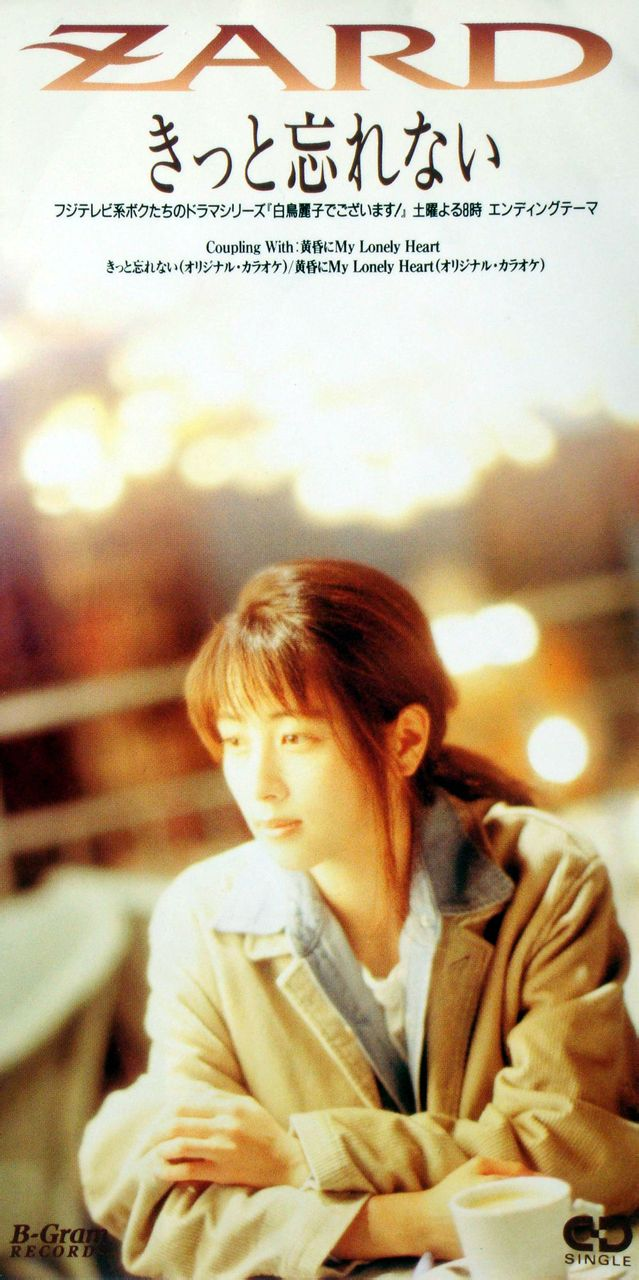
\includegraphics[width=0.3\textwidth]{S10.jpg}}

\large{

きっと\ruby{忘}{わす}れない \ruby{眩}{まぶ}しいまなざしを

\ruby{信}{しん}じたい \ruby{信}{しん}じてる

あなたが\ruby{変}{か}わらぬように
\\

every day  every night \ruby{泣}{な}いたりしたけど

\ruby{誰}{だれ}にも\ruby{話}{はな}せなくて

\ruby{無器用}{ぶきよう}だけど せいいっぱいあなたを

\ruby{愛}{あい}した あの\ruby{季節}{きせつ}

\ruby{暮}{く}れゆく\ruby{都会}{まち} あふれる\ruby{人波}{ひとなみ}

\ruby{今}{いま}にも\ruby{笑顔}{えがお}であなたが\ruby{現}{あらわ}れそうで
\\

きっと\ruby{忘}{わす}れない また\ruby{冬}{ふゆ}が\ruby{来}{き}ても

\ruby{想}{おも}い\ruby{出}{で} \ruby{抱}{だ}きしめていたいから

\ruby{空}{そら}の\ruby{彼方}{かなた}へと\ruby{悲}{かな}しみ\ruby{吹}{ふ}き\ruby{飛}{と}ばせ

\ruby{信}{しん}じたい \ruby{信}{しん}じてる

あなたが\ruby{変}{か}わらぬように
\\

\ruby{別}{わか}れは\ruby{粉雪}{こなゆき} \ruby{淋}{さび}しさが\ruby{胸}{むね}に

\ruby{積}{つ}もる「また\ruby{会}{あ}いたい」

どうして あの\ruby{時}{とき} \ruby{傷}{きず}つけあったのだろう

\ruby{強}{つよ}がるしかなくて

\ruby{星}{ほし}くずの\ruby{中}{なか} \ruby{間}{ま}に\ruby{合}{あ}うように

\ruby{渋滞}{じゅうたい}\ruby{抜}{ぬ}けて \ruby{送}{おく}ってくれたね いつも
\\

きっと\ruby{忘}{わす}れない \ruby{眩}{まぶ}しいまなざしを

せつない\ruby{約束}{やくそく}が\ruby{痛}{いた}いけど

\ruby{遠}{とお}く\ruby{離}{はな}れても \ruby{心}{こころ}は\ruby{止}{と}まらない

あきらめたい あきらめない

\ruby{孤独}{こどく}が\ruby{ドア}{Door}を\ruby{叩}{たた}く
\\

きっと\ruby{忘}{わす}れない また\ruby{冬}{ふゆ}が\ruby{来}{き}ても

\ruby{想}{おも}い\ruby{出}{で} \ruby{抱}{だ}きしめていたいから

\ruby{空}{そら}の\ruby{彼方}{かなた}へと\ruby{悲}{かな}しみ\ruby{吹}{ふ}き\ruby{飛}{と}ばせ

\ruby{信}{しん}じたい \ruby{信}{しん}じてる

あなたが\ruby{変}{か}わらぬように

}